\section{Introduction}
Composite materials offer improved strength, stiffness, fatigue, corrosion resistance, etc. over
conventional materials, and are widely used as materials for applications ranging from the automotive to shipbuilding
industry, electronic packaging to golf clubs, and medical equipment to homebuilding. However, the high
cost of fabrication of composites is a critical drawback to its application. For example, the
graphite/epoxy composite part may cost as much as $650$ to $900$ per kilogram. In contrast, the price
of glass/epoxy is about 2.5 times less. Manufacturing techniques such as sheet molding compounds and
structural reinforcement injection molding are used to lower the  costs for manufacturing automobile parts.
An alternative approach is using hybrid composite materials.


The mechanical performance of a laminate composite is affected by a wide range of factors such as the
thickness, material, and orientation of each laminae. Because of manufacturing limitations, all these
variables are usually limited to a small set of discrete values. For example, the ply thickness is fixed,
and ply orientation angles are limited to a set of angles such as 0, 45, and 90 degrees in practice. So
the search process for the optimal design is a discrete optimization problem that can be solved by the
GA. To tailor a laminate composite, the GA has been successfully applied to solve laminate design
problems\cite{riche1993optimization,nagendra1996improved,sadagopan1998application,todoroki1998stacking,liu2000permutation,sivakumar1998optimum,walker2003technique,lin2004stacking,kang2005minimum,murugan2007target,akbulut2008optimum}.
The GA simulates the process of natural evolution, including selection, crossover, and mutation
according to Darwin's principle of ''survival of the fittest''. The known advantages of GAs are the
following: (i): GAs are not easily trapped in local optima and can obtain the global
optimum. (ii): GAs do not need gradient information and can be applied to discrete optimization
problems. (iii): GAs can not only find the optimal value in the domain but also maintain a
set of optimal solutions. However, the GA also has some disadvantages, for example, the GA
needs to evaluate the target functions many times to achieve the optimization, and the cost of the
search process is high. The GA consists of some basic parts, the coding of the design variable,
the selection strategy, the crossover operator, the mutation operator, and how to deal with constraints. For the
variable design part, there are two methods to deal with the representation of design variables, namely,
binary string and real value representation\cite{riche1993optimization,todoroki1998stacking}.
Michalewicz\cite{zbigniew1996genetic} claimed that the performance of floating-point representation was
better than binary representation in the numerical optimization problem. Selection strategy plays a
critical role in the GA, which determines the convergence speed and the diversity of the population. To
improve search ability and reduce search costs, various selection methods have been invented, and they
can be divided into four classes: proportionate reproduction, ranking, tournament, and
genitor(or ''steady state'') selection. In the optimization of laminate composite design, the roulette
wheel\cite{riche1993optimization,seresta2007optimal}, where the possibility of an individual to be
chosen for the next generation is proportional to the fitness.
Soremekun et al.\cite{soremekun2001composite} showed that the generalized elitist strategy outperformed a
single individual elitism in some special cases.

Data structure, repair strategies, and penalty functions\cite{le1995improved} are the most commonly used
approaches to resolve constrained problems in the optimization of composite structures. Symmetric
laminates are widely used in practical scenarios, and data structures can be used to fulfill symmetry
constraints, which consists of coding half of the laminate and considering the rest with the
opposite orientation. Todoroki\cite{todoroki1998stacking} introduced a repair strategy that can scan the chromosome and
repair the gene on the chromosome if it does not satisfy the contiguity constraint. The comparison of
repair strategies in a permutation GA with the same orientation was presented by Liu et al.\cite{liu2000permutation}, and it
showed that the Baldwinian repair strategy can substantially reduce the cost of constrained optimization.
Haftka and Todoroki\cite{riche1993optimization} used the GA to solve the laminate stacking sequence problem using a penalty function subject to
buckling and strength constraints.

In typical engineering applications, composite materials are under very complicated loading
conditions, not only inplane loading but also out-of-plane loading. Most of the studies on the
optimization of the laminate composite material minimized the
thickness\cite{abu1998optimum,walker2003technique},
weight\cite{fang1993design,deka2005multiobjective,park2008improved}, and cost and
weight\cite{deka2005multiobjective,omkar2008artificial}, or maximized the static strength of
the composite laminates for a targeted
thickness\cite{walker2003technique,lin2004stacking,kim2007development,gholami2020multi}. 
In the present study,
the cost and weight of laminates are minimized by modifying the objective function.

To check the feasibility of a laminate composite by imposing a strength constraint, failure
analysis of a laminate is performed by applying suitable failure criteria. The failure criteria of
laminated composites can be classified into three classes: non-interactive theories (e.g., maximum
strain), interactive theories (e.g., Tsai-wu), and partially interactive theories (e.g., Puck failure
criterion). Previous researchers adopted the first-ply-failure approach using Tsai-wu
failure
theory\cite{massard1984computer,reddy1987first,fang1993design,soeiro1994multilevel,pelletier2006multi,jadhav2007parametric,omkar2008artificial,choudhury2019failure},
Tsai-Hill\cite{martin1987optimum,soares1995discrete}, the maximum stress\cite{watkins1987multicriteria}, or the maximum strain\cite{watkins1987multicriteria}
static failure criteria. Akbulut\cite{akbulut2008optimum} used the GA to minimize the thickness of composite laminates with
Tsai-Hill and maximum stress failure criteria, and the advantage of this method is it avoids spurious
optima. Naik et al.\cite{naik2008design}
minimized the weight of laminated composites under restrictions with a
failure mechanism-based criterion based on the maximum strain and Tsai-wu. In the present study, Tsai-wu
Static failure criteria are used to investigate the feasibility of a laminate composite.

\section{Stress and Strain in a Laminate}
\begin{figure*}[!htb]
	\centering
	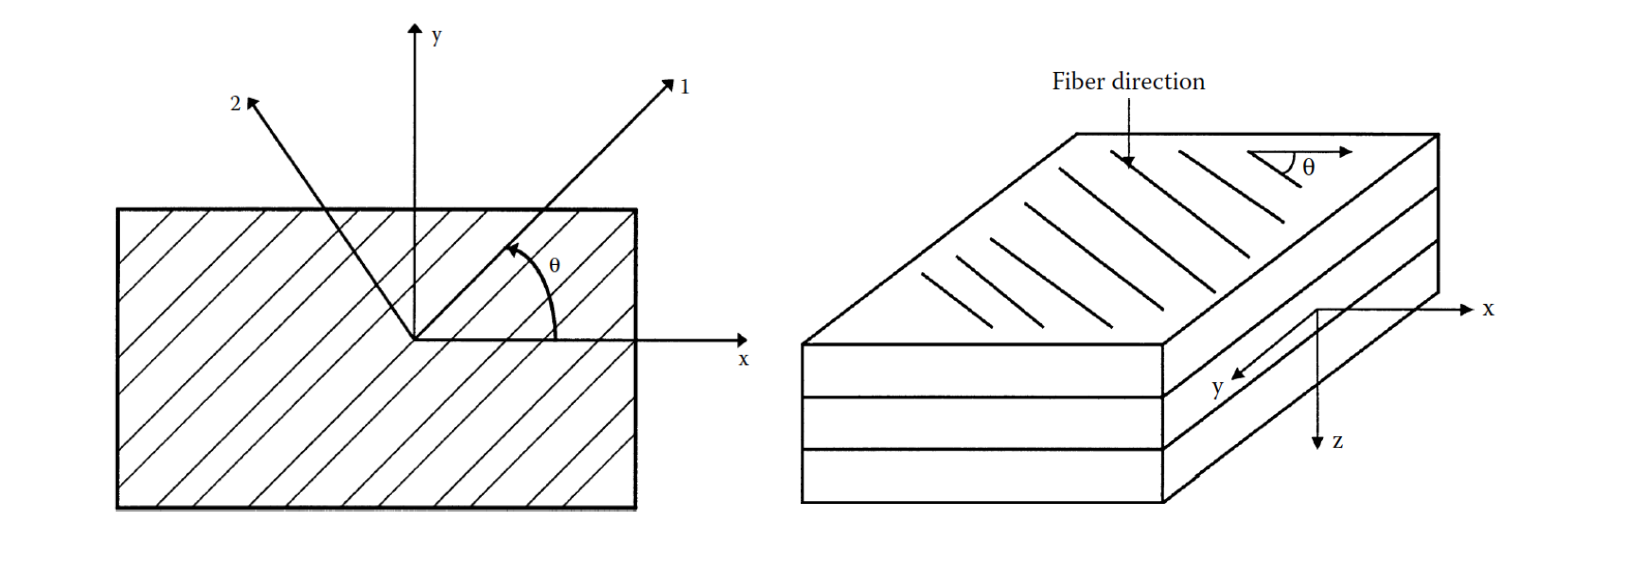
\includegraphics[width=\linewidth]{\ROOT/fig/lamina_local_global_axes.png}
	\caption{Local and global axes of an angle lamina.}
  	\label{fig:lamina}
\end{figure*}

\begin{figure} \centering
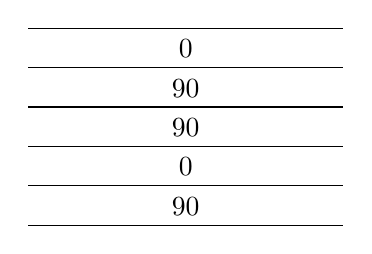
\begin{tikzpicture}
	\draw (0,0) -- (4,0);
	\draw (0,-0.5) -- (4,-0.5) node[midway, above] {$0$};
	\draw (0,-1) -- (4,-1) node[midway, above] {$90$} ;
	\draw (0,-1.5) -- (4,-1.5) node[midway, above] {$90$};
	\draw (0,-2) -- (4,-2) node[midway, above] {$0$};
	\draw (0,-2.5) -- (4,-2.5) node[midway, above] {$90$};
\end{tikzpicture}
\caption{Model for cross ply laminate.}
\end{figure}

A laminate structure consists of multiple lamina bonded together through their thickness.
Considering a laminate composite plate that is symmetric to its middle plane subject to in-plane
loading of extension, shear, bending and torsion, the classical lamination theory (CLT) is taken to
calculate the stress and strain in the local and global axes of each ply, as shown in
Fig.~\ref{fig:lamina}.

\begin{table*}[ht]
\caption{Comparison of the graphite/epoxy and glass/epoxy properties}
\centering
\begin{adjustbox}{width=1\textwidth}
\label{tab:mat}
\begin{tabular}{lcccc}
\toprule
Property								   & Symbol				  & Unit  &  Graphite/Epoxy  &  Glass/Epoxy   \\
\midrule
Longitudinal elastic modulus			   & $E_1$				  & GPa   &  181             &  38.6           \\
Traverse elastic modulus				   & $E_2$				  & GPa   &  10.3            &  8.27           \\
Major Poisson's ratio					   & $v_{12}$			  &       &  0.28            &  0.26           \\
Shear modulus							   & $G_{12}$			  & GPa   &  7.17            &  4.14           \\
Ultimate longitudinal tensile strength     & $(\sigma_1^T)_{ult}$ & MP    &  1500            &  1062            \\
Ultimate longitudinal compressive strength & $(\sigma_1^C)_{ult}$ & MP    &  1500            &  610             \\
Ultimate transverse tensile strength       & $(\sigma_2^T)_{ult}$ & MPa   &  40              &  31              \\
Ultimate transverse compressive strength   & $(\sigma_2^C)_{ult}$ & MPa   &  246             &  118              \\
Ultimate in-plane shear strength           & $(\tau_{12})_{ult}$  & MPa   &  68              &  72               \\
Density                                    & $\rho$               & $g/cm^3$  &  1.590           &  1.903               \\
Cost                                       &                      &           &  2.5             &  1               \\
\bottomrule
\end{tabular}
\end{adjustbox}
\end{table*}



\subsection{Stress and Strain in a Lamina}
For a single lamina, the stress-strain relation in local axis 1-2 is:
\begin{equation}
    \begin{bmatrix}
        \sigma _1\\
        \sigma _2\\
        \tau_{12}
    \end{bmatrix}
    =
    \begin{bmatrix}
        Q_{11} & Q_{12} & 0\\
        Q_{12} & Q_{22} & 0\\
        0      &  0     & Q_{66}
    \end{bmatrix}
    \begin{bmatrix}
        \varepsilon_1\\
        \varepsilon_2\\\gamma_{12}
	\end{bmatrix} \textstyle{,}
\end{equation}
where $Q_{ij} $ are the stiffnesses of the lamina that are related

to engineering elastic constants given by
\begin{equation}
    \begin{split}
    &Q_{11}=\frac{E_1}{1-v_{12}v_{21}}\textstyle{,}\\
    &Q_{22}=\frac{E_2}{1-v_{12}v_{21}}\textstyle{,}\\
    &Q_{66}=G_{12}\textstyle{,}\\
    &Q_{12}=\frac{v_{21}E_2}{1-v_{12}v_{21}}\textstyle{,}\\
    \end{split}
\end{equation}

where $E_1, E_2, v_{12}, G_{12} $ are four independent engineering elastic constants, which are defined as follows: $E_1 $ is the longitudinal Young's modulus, $E_2 $ is the transverse Young's modulus, $v_{12} $ is the major Poisson's ratio, and $G_{12} $ is the in-plane shear modulus.

Stress strain relation in the global x-y axis:
\begin{equation}
	\left[\begin{array}{l}\sigma _{x} \\ 
		\sigma _{y} \\ 
		\tau_{xy}
	\end{array}\right]=
	\left[\begin{array}{lll}
		\bar{Q}_{11} & \bar{Q}_{12} & \bar{Q}_{16}\\ 
	    \bar{Q}_{12} & \bar{Q}_{22} & \bar{Q}_{26} \\ 
	    \bar{Q}_{16} & \bar{Q}_{26} &\bar{Q}_{66}
	\end{array}\right]\left[\begin{array}{l}\varepsilon_{x} \\ 
	\varepsilon_{y}\\ \gamma_{x y}\end{array}\right] \textstyle{,}
\end{equation}
where

\begin{equation}
	\begin{array}{l}
		\resizebox{.35\textwidth}{!}{$\bar{Q}_{11}=Q_{11} c^{4}+Q_{22} s^{4}+2\left(Q_{12}+2
		Q_{66}\right) s^{2} c^{2}$} \textstyle{,}\\
		\resizebox{.35\textwidth}{!}{$\bar{Q}_{12}=\left(Q_{11}+Q_{22}-4 Q_{66}\right) s^{2}
		c^{2}+Q_{12}\left(c^{4}+s^{2}\right)$} \textstyle{,}\\
		\resizebox{.35\textwidth}{!}{$\bar{Q}_{22}=Q_{11} s^{4}+Q_{22} c^{4}+2\left(Q_{12}+2
		Q_{66}\right) s^{2} c^{2}$} \textstyle{,}\\
		\resizebox{.4\textwidth}{!}{$\bar{Q}_{16}=\left(Q_{11}-Q_{12}-2 Q_{66}\right) c^{3} s-\left(Q_{22}-Q_{12}-2Q_{66}\right) s^{3} c$}\textstyle{,}
		 \\ 
		\resizebox{.4\textwidth}{!}{$\bar{Q}_{26}=\left(Q_{11}-Q_{12}-2 Q_{66}\right) c s^{3}-\left(Q_{22}-Q_{12}-2 Q_{66}\right)c^{3} s$}\textstyle{,}
		 \\ 
	\resizebox{.4\textwidth}{!}	{$\bar{Q}_{66}=\left(Q_{11}+Q_{22}-2 Q_{12}-2 Q_{66}\right)
	s^{2}c^{2}+Q_{66}\left(s^{4}+c^{4}\right)$}\textstyle{.}\\
	\end{array}
\end{equation}


The c and s denote $cos\theta $ and $sin\theta $, respectively.

The local and global stresses in an angle lamina are related

to each other through the angle of the lamina $\theta $
\begin{equation}\left[\begin{array}{l}\sigma _{1} \\ \sigma _{2} \\ \tau_{12}\end{array}\right]=[T]\left[\begin{array}{l}\sigma _{x} \\ \sigma _{y} \\\tau_{xy}\end{array}\right]
\end{equation}

where
\begin{equation}[T]=\left[\begin{array}{ccc}c^{2} & s^{2} & 2 s c \\ s^{2} & c^{2} & -2 s c \\ -s c & s c &c^{2}-s^{2}\end{array}\textstyle{.}\right] 
\end{equation}



\subsection{Stress and Strain in a Laminate}
\begin{equation} \label{eq:force_and_moments}
	\begin{array}{l}
		\begin{aligned}
	\begin{bmatrix}
		N_x \\
		N_y \\
		N_{xy}
	\end{bmatrix}
	&=
	\begin{bmatrix}
		A_{11} & A_{12} & A_{16} \\
		A_{12} & A_{22} & A_{26} \\
		A_{16} & A_{26} & A_{66} 
	\end{bmatrix}
    \begin{bmatrix}
		\varepsilon_x^0 \\
        \varepsilon_y^0 \\
		\gamma_{xy}^0
    \end{bmatrix}   \\
	&+               
	\begin{bmatrix}
		B_{11} & B_{12} & B_{16} \\
		B_{11} & B_{12} & B_{16} \\
		B_{16} & B_{26} & B_{66} 
	\end{bmatrix}
	\begin{bmatrix}
		k_x \\
		k_y \\
		k_{xy} 
	\end{bmatrix}  \\
\end{aligned} \\ \\
\begin{aligned}
	\begin{bmatrix}
		M_x \\
		M_y \\
		M_{xy}
	\end{bmatrix}
	&=
	\begin{bmatrix}
		B_{11} & B_{12} & B_{16} \\
		B_{12} & B_{22} & B_{26} \\
		B_{16} & B_{26} & B_{66} 
	\end{bmatrix}
    \begin{bmatrix}
		\varepsilon_x^0 \\
        \varepsilon_y^0 \\
		\gamma_{xy}^0
    \end{bmatrix} \\ 
	&+  
	\begin{bmatrix}
		D_{11} & D_{12} & D_{16} \\
		D_{11} & D_{12} & D_{16} \\
		D_{16} & D_{26} & D_{66} 
	\end{bmatrix}
	\begin{bmatrix}
		k_x \\
		k_y \\
		k_{xy} 
	\end{bmatrix}
\end{aligned}
	\end{array}
\end{equation}


$N_x,N_y $  - normal force per unit length

$N_{xy} $  - shear force per unit length

$M_x, M_y $ - bending moment per unit length

$M_{xy} $  - twisting moments per unit length

$\varepsilon^{0}, k $- mid-plane strains and curvature of a laminate in x-y coordinates

The mid-plane strain and curvature is given by
\begin{equation}
    \begin{split}
	&A_{ij}=\sum_{k=1}^{n}(\overline{Q_{ij}})_k(h_k-h_{k-1})  i=1,2,6, j=1,2,6 \textstyle{,}\\
	&B_{ij}=\frac{1}{2}\sum_{k=1}^{n}(\overline{Q_{ij}})_k(h^2_k - h_{k-1}^2)  i=1,2,6, j=1,2,6 \textstyle{,}\\
	&D_{ij}=\frac{1}{3}\sum_{k=1}^{n}(\overline{Q_{ij}})_k(h^3_k - h_{k-1}^3) i=1,2,6, j=1,2,6 \textstyle{,}\\
    \end{split}
\end{equation}

where the [A], [B], and [D] matrices are called the extensional, coupling, and bending stiffness matrices.

\section{Failure Theory}

\subsection{Failure Process}
A laminate will fail under increasing mechanical loading; however, the procedure of laminate failure may not
be catastrophic.
 In some cases, some layers fail first, and the rest are able to continue to take additional loading
 until all the plies fail. A ply is fully discounted when a ply fails; then, the ply is replaced
by a near-zero stiffness and strength. 
The procedure for finding the first ply failure in the present
study follows the fully discounted method:

\begin{enumerate}
\item Compute the reduced stiffness matrix [Q] referred to as the local axis for each ply using its four engineering elastic constants $E_1 $, $E_2 $, $E_{12} $, and $G_{12} $.

\item Calculate the transformed reduced stiffness $[\bar{Q}] $ referring to the global coordinate system (x, y) using the reduced stiffness matrix [Q] obtained in step 1 and the ply angle for each layer.

\item  Given the thickness and location of each layer, the three laminate stiffness matrices [A], [B], and [D] are determined.

\item  Apply the forces and moments, $[N]_{xy}, [M]_{xy} $ solve
Equation \ref{eq:force_and_moments}, and calculate the middle plane strain $[\sigma ^{0}]_{xy} $ and curvature $[k]_{xy} $.

\item Determine the local strain and stress of each layer under the applied load.

\item  Use the ply-by-ply stress-strain and related failure theories to determine the strength ratio.
\end{enumerate}

\subsection{Tsai-wu Failure Theory}

Many different theories about the failure of an angle lamina have been developed for a
unidirectional lamina, such as the maximum stress failure theory, maximum strain failure theory,
Tsai-Hill failure theory, and Tsai-Wu failure theory. The failure theories of a lamina are based on
the stresses in the local axes in the material. There are four normal strength parameters and one shear
stress for a unidirectional lamina. The five strength parameters are:

$(\sigma _1^{T})_{ult}= $ ultimate longitudinal tensile strength

$(\sigma _1^{C})_{ult}= $ ultimate longitudinal compressive strength

$(\sigma _2^{T})_{ult}= $ ultimate transverse tensile strength

$(\sigma _2^{C})_{ult}= $ ultimate transverse compressive strength 

$(\tau_{12})_{ult}= $ and ultimate in-plane shear strength

In the present study, Tsai-wu failure theory is taken to decide whether a lamina fails,
because this theory is more general than the Tsai-Hill failure theory, which considers two
different situations, the compression and tensile strengths of a lamina. A lamina is considered to fail
if \begin{equation} \label{eq:tsai_wu}
\begin{split}
	H_1 \sigma_1  & + H_2 \sigma_2 + H_6 \tau_{12} + H_{11}\sigma_1^2 + H_{22} \sigma_2^2 \\
				  & + H_{66}  \tau_{12}^2 + 2H_{12}\sigma_1\sigma_2 < 1
\end{split}
\end{equation}

is violated, where

\begin{equation} \label{eq:sr}S R=\frac{\text {Maximum Load}}{\text {Load Applied}}
\end{equation}

The maximum load refers to that can be applied using Tsai-wu failure theory.

